\documentclass{beamer}

\usetheme{JuanLesPins}

% --- Languages & Fonts ---
\usepackage{polyglossia}

\newfontfamily\greekfont[Script=Greek]{Linux Libertine O}
\newfontfamily\greekfontsf[Script=Greek]{Linux Libertine O}
\newfontfamily\greekfonttt[Script=Greek]{Linux Libertine Mono O}

\setdefaultlanguage{greek}
\setotherlanguage{english}

\usepackage{caption}
\captionsetup[figure]{font=scriptsize}

% --- Cover ---
\title{Concordia}
\subtitle{Αυτόνομο κοινωνικό δίκτυο\\βασισμένο σε τεχνολογίες αποκέντρωσης}

\definecolor{concordia}{RGB}{11, 37, 64}

\newcommand{\keyword}[1]{\textbf{\textcolor{concordia}{#1}}}

\author{Νικολαΐδης Παναγιώτης \and Φανάκης Απόστολος}

\institute{
	Αριστοτέλειο Πανεπιστήμιο Θεσσαλονίκης\newline
	Τμήμα Ηλεκτρολόγων Μηχανικών και Μηχανικών Υπολογιστών
}

\date{Θεσσαλονίκη \the\year}

\begin{document}

\frame{\titlepage}

\begin{frame}
	\frametitle{Table of Contents}
	\tableofcontents
\end{frame}

\section{Ορισμός του προβλήματος}
\begin{frame}
	\frametitle{Ορισμός του προβλήματος}
\end{frame}

\section{Στόχος της εργασίας}
\begin{frame}
	\frametitle{Στόχος της εργασίας}
\end{frame}

\section{Επισκόπηση Εφαρμογής}
\begin{frame}
	\frametitle{Επισκόπηση Εφαρμογής}
\end{frame}

\section{Τεχνολογική Στοίβα}
\begin{frame}
	\frametitle{Τεχνολογική Στοίβα}
	\centering
	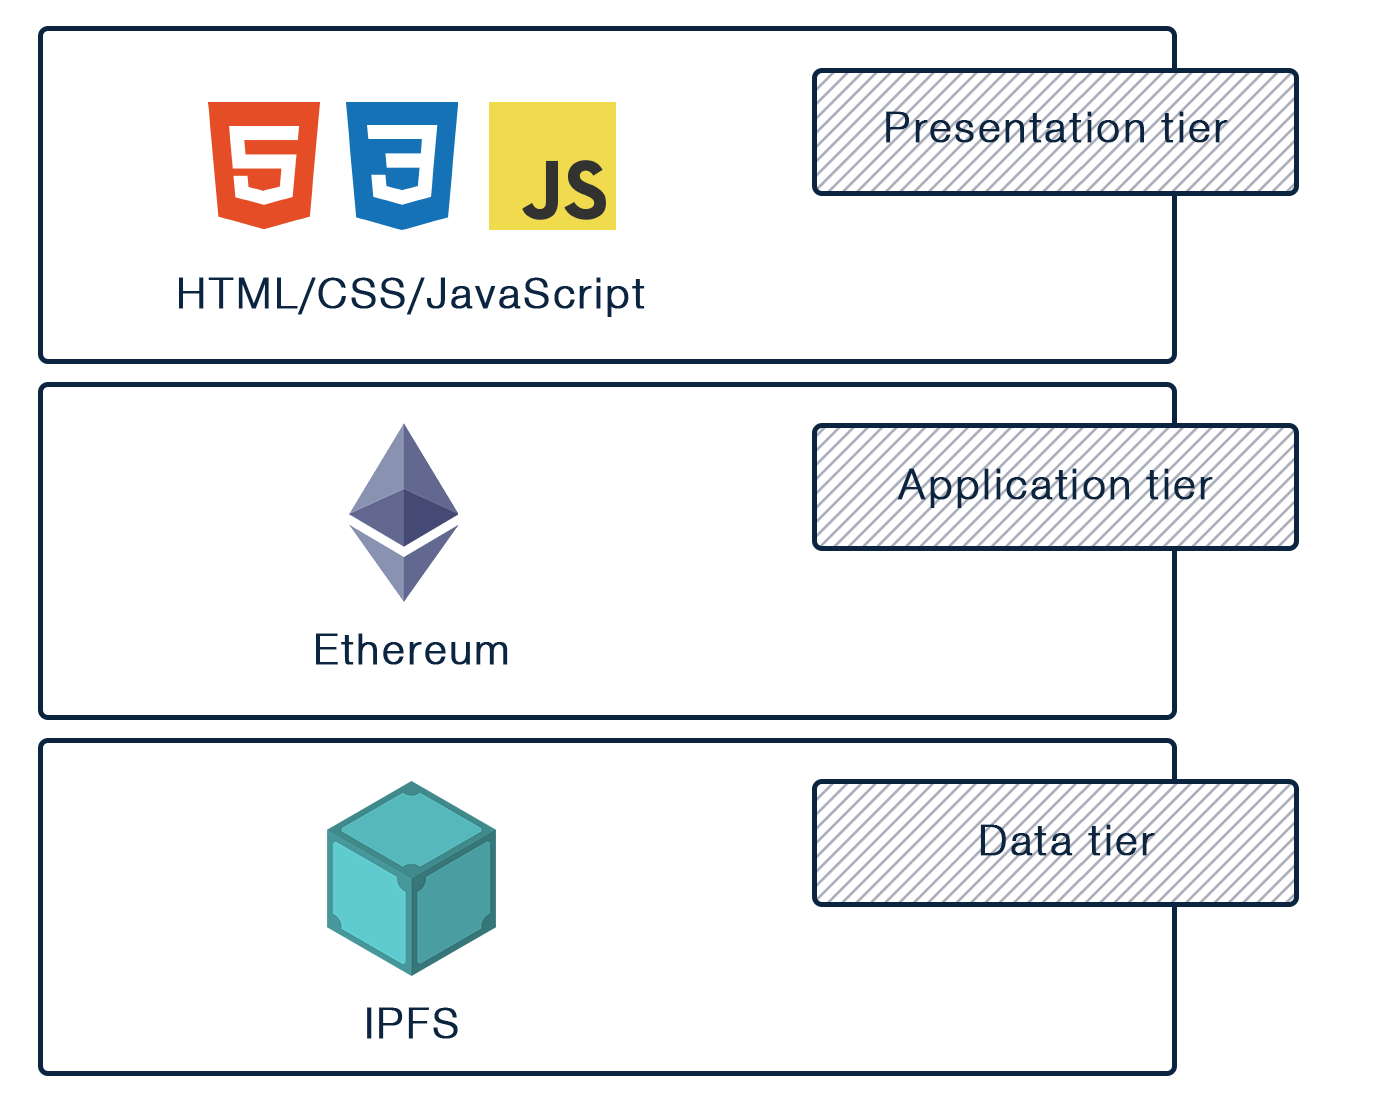
\includegraphics[scale=0.15]{assets/figures/technology-stack}
\end{frame}

\note{
	Ξεκινώντας τη σχεδίαση της πλατφόρμας, πραγματοποιήσαμε έρευνα για την επιλογή της τεχνολογικής στοίβας. Αυτή αποφασίσαμε να ακολουθήσει μία προσαρμοσμένη για τα δεδομένα μορφή τριμερούς διάταξης και έτσι να χωριστεί σε τρία λογικά επίπεδα, όπως φαίνονται στη διαφάνεια.
	Το πρώτο επίπεδο, δηλαδή το Presentation tier, αποτελεί τη διεπαφή του χρήστη, μέσω της οποίας εκείνος αλληλεπιδρά με την εφαρμογή. Αυτό αναπτύχθηκε ως μία κλασική client-side web application σε HTML/CSS/JavaScript με τη χρήση σύγχρονων web framework και δε θα το αναλύσουμε ιδιαίτερα.
	Το δεύτερο επίπεδο, δηλαδή το Application tier, είναι εκείνο στο οποίο πραγματοποιείται η επεξεργασία της εφαρμογής. Εδώ επιλέχθηκαν να χρησιμοποιηθούν το blockchain και τα smart contract και συγκεκριμένα η πλατφόρμα του Ethereum.
	Τέλος, για το τρίτο επίπεδο, δηλαδή το Data tier, το οποίο είναι υπεύθυνο για την αποθήκευση του κύριου όγκου των δεδομένων, επιλέχθηκε το IPFS.
}

\section{Ethereum}
\begin{frame}
	\frametitle{Ethereum}
\end{frame}

\section{IPFS}
\begin{frame}
	\frametitle{IPFS}
\end{frame}

\section{Αρχιτεκτονική προγραμματιστικού περιβάλλοντος}
\begin{frame}
	\frametitle{Αρχιτεκτονική προγραμματιστικού περιβάλλοντος}
\end{frame}

\section{Μέθοδοι και Χρονοδιάγραμμα Υλοποίησης}
\begin{frame}
	\frametitle{Μέθοδοι και Χρονοδιάγραμμα Υλοποίησης}
\end{frame}

\section{Δυνατότητες Εφαρμογής}
\begin{frame}
	\frametitle{Δυνατότητες Εφαρμογής}
\end{frame}

\section{Συμπεράσματα}
\begin{frame}
	\frametitle{Συμπεράσματα}
	\vspace{-\baselineskip}
	\begin{center}
		
\includegraphics[width=.1\paperwidth]{assets/figures/concordia-logo}
	\end{center}
	\textbf{Concordia} - μία πλήρως αποκεντρωμένη αυτόνομη κοινωνική πλατφόρμα ...με ορισμένα εμπόδια:
	\begin{itemize}
		\item Πρώιμες τεχνολογίες
		\item Ethereum - τέλη συναλλαγών, συγκράτηση χρηστών, κλιμακοθετησιμότητα
		\item IPFS υβριδικό ως προς την ανακάλυψη κόμβων
	\end{itemize}
\end{frame}

\note{
	Καταλήγουμε έτσι στα συμπεράσματα της εργασίας.
	
	Όσον αφορά στον αρχικό στόχο, η πιλοτική μας εφαρμογή αποδεικνύει ότι ο σχεδιασμός μιας πλατφόρμας που να εκπληρώνει τους στόχους που τέθηκαν είναι εφικτός. Είναι δηλαδή εφικτή τόσο η κατοχύρωση της ελευθερίας του λόγου των χρηστών, όσο και η εξασφάλιση αυθεντικών δημοκρατικών διαδικασιών, μέσω των τεχνολογιών που επιλέχθηκαν.
	
	Ωστόσο, πρέπει να πούμε ότι υπάρχουν ορισμένα σημαντικά εμπόδια.
	
	Πρώτα απ' όλα και οι δύο τεχνολογίες είναι ακόμα πρώιμες. Αυτό σημαίνει ότι έχουμε ακόμα beta versions, διάφορες ελλείψεις και τεχνικά ζητήματα που δεν έχουν λυθεί.

	Όσον αφορά στο Ethereum, όπως έχουν τα πράγματα με τα τέλη των συναλλαγών και την \textit{ανάγκη χρήσης πρόσθετου λογισμικού} για τη σύνδεση με το blockchain, κάνουν ιδιαίτερα δύσκολο τόσο να υιοθετηθεί από τους χρήστες, όσο και αυτοί να παραμείνουν σε αυτό. Επίσης, πέρα από τη συγκράτηση των χρηστών, υπάρχει το θέμα της κλιμακοθετησιμότητας, με την έννοια ότι αυτή τη στιγμή επιτρέπονται σχετικά λίγες συναλλαγές ανά δευτερόλεπτο επί του Ethereum.
	
	Από την άλλη υπάρχει προς το παρόν το πρόβλημα ότι ως προς την ανακάλυψη κόμβων το IPFS λειτουργεί υβριδικά, απαιτείται δηλαδή μία σύνδεση με signalling nodes για την ανακάλυψη των κατάλληλων peer.
}
\section{Ανοιχτά Θέματα}
\begin{frame}
	\frametitle{Ανοιχτά Θέματα}
	\begin{itemize}
		\item Διαχείριση των τελών του Ethereum
		\item Διανομή των Ethereum token
		\item Εναλλακτικά συστήματα ψηφοφορίας
		\item Συστήματα απόδοσης εμπιστοσύνης
	\end{itemize}
\end{frame}

\note{
	Έτσι, φτάνουμε στα ανοιχτά θέματα.
	
	Το πρώτο και σημαντικότερο είναι η διαχείριση των τελών στις συναλλαγές του Ethereum. Αυτό που προτείνουμε και είναι γενικά η τάση που επικρατεί είναι η χρήση μετασυναλλαγών. Στην περίπτωσή μας αυτό θα σήμαινε π.χ. ότι η πληρωμή των τελών θα προωθείται από τον χρήστη στην κοινότητα που ανήκει.
	
	Ένα δεύτερο ζήτημα είναι η δημιουργία μηχανισμών για την ανώνυμη διανομή των token στους χρήστες. Αν και στην υλοποίησή μας αφήσαμε ανοιχτή τη διαδικασία διανομής των token στην εκάστοτε κοινότητα, θα πρέπει να τονίσουμε ότι σχετικά πρόσφατα άρχισαν να εμφανίζονται υλοποιήσεις στο Ethereum που μπορούν να ενσωματωθούν και που την απλοποιούν κατά πολύ, επιτρέποντας την ανώνυμη μετακίνηση token από διεύθυνση σε διεύθυνση.
	
	Επίσης, οι διαδικασίες των ψηφοφοριών μπορούν να επεκταθούν και να ορίζονται αυθαίρετα από την κάθε κοινότητα. Για παράδειγμα να υπάρχει επιλογή για ψηφοφορία με σειρά προτίμησης ή για έμμεση ψηφοφορία.
	
	Τέλος, μπορούν να χτιστούν συστήματα απόδοσης εμπιστοσύνης για τους χρήστες, τα οποία να λειτουργούν κυρίως συμπληρωματικά με τα θέματα των τελών και των ψηφοφοριών. Για παράδειγμα σε μία κοινότητα ένας χρήστης να απαλλάσσεται από τέλη εάν περάσει ένα όριο εμπιστοσύνης ή η ισχύς της ψήφου του να ορίζεται από αυτήν.
}


\end{document}
